
\section{\label{part:3}Détermination de la loi de mouvement du système perturbé }
\begin{obj}
Élaborer le modèle dynamique et déterminer la loi de mouvement du système perturbé afin de mettre en évidence la nécessité d'ajouter une commande active au système pour assurer le respect de l'exigence 1.2. relative à la position en mouvement du cahier des charges.
\end{obj}

\ifprof
\else
Dans cette partie, l'étude est conduite avec les hypothèses suivantes :

\begin{itemize}
  \item les quatre liaisons pivots et la liaison glissière sont parfaites ;
  \item la modélisation est plane ;
  \item le système est perturbé par l'utilisateur au niveau de la glissière (figure~\ref{fig:04}) et cette perturbation est modélisée par une fonction sinusoïdale $z_{\text {pert }}(t)=Z_{0} \sin (\omega t)$ avec l'amplitude $Z_{0}$ et la pulsation $\omega$ constantes ;
  \item à l'instant initial de cette étude, la nacelle gyrostabilisée (figure~\ref{fig:04}) est à l'équilibre.
\end{itemize}
\fi

\subsection{Détermination de la loi de mouvement}
%Q 13. 
\question{\label{q:13} En isolant l'ensemble constitué de la nacelle gyrostabilisée (3) et de l'appareil photo (4) (formant un seul solide) et en traduisant une équation scalaire issue du principe fondamental de la dynamique, donner l'équation différentielle traduisant la loi de mouvement du système. Écrire l'équation différentielle sous la forme
$
\ddot{\alpha}=C_{1} \ddot{z}_{\text {pert }} \cos \alpha+C_{2} \cos \alpha+C_{3} F_{r} \sin (\beta-\alpha)
$
en précisant l'expression des trois constantes $C_{1}, C_{2}$ et $C_{3}$ en fonction de $m_{34}, L$ et $g$.}
\ifprof
\begin{corrige}
En reprenant le raisonnement de la partie précédente, on isole \{(3)+(4)\} et on applique le TRD en projection sur $\vect{z_2}$.

Calculons $\vectrd{3}{0}=m_{34}\vectg{G}{3}{0}$ =$m_{34}\left[\dfrac{\dd \vectv{G}{3}{0}}{\dd t}\right]_{\rep{0}}$.

De plus, $\vectv{G}{3}{0}=\left[\dfrac{\dd \vect{OG}}{\dd t}\right]_{\rep{0}}$
$=\left[\dfrac{\dd \left(y_A\vect{y_0}+z_{\text{pert}}\vect{z_0}+L\vect{y_2}+y_G\vect{y_0}+z_{G}\vect{z_0}\right)}{\dd t}\right]_{\rep{0}}$

$=\left[\dfrac{\dd \left(z_{\text{pert}}\vect{z_0}+L\vect{y_2}\right)}{\dd t}\right]_{\rep{0}}$
$=\dot{z}_{\text{pert}}\vect{z_0}+L\dot{\alpha}\vect{z_2}$.

Donc, $\vectg{G}{3}{0} = \ddot{z}_{\text{pert}}\vect{z_0}+L\ddot{\alpha}\vect{z_2}-L\dot{\alpha}^2\vect{y_2}$.

Ainsi $\vectrd{3}{0}\cdot\vect{z_2} = m_{34}\ddot{z}_{\text{pert}}\cos\alpha+Lm_{34}\ddot{\alpha}$.

Le TRD en projection sur $\vect{z_2}$ donne alors 
$m_{34}\ddot{z}_{\text{pert}}\cos\alpha+Lm_{34}\ddot{\alpha} 
= -m_{34} g\cos\alpha -F_r\sin\left(\alpha-\beta \right)$.

Soit 
$$\boxed{\ddot{\alpha} 
= - \dfrac{g}{L}\cos\alpha +\dfrac{F_r}{Lm_{34}}\sin\left(\beta - \alpha \right)-\dfrac{1}{L}\ddot{z}_{\text{pert}}
\cos\alpha}$$

En identifiant, on a $C_1=-\dfrac{1}{L}$, $C_2 = -\dfrac{g}{L}$ et $C_3 = \dfrac{1}{Lm_{34}}$.
\end{corrige}
\else
\fi

\ifprof
\else
L'équation différentielle traduisant la loi de mouvement du système est du second ordre. Pour résoudre numériquement une telle équation différentielle, elle peut être réécrite sous la forme d'une équation différentielle vectorielle du premier ordre. On définit pour cela, le vecteur $A(t)$ par

$$
A(t)=\left(\begin{array}{c}
\alpha(t) \\
\dot{\alpha}(t)
\end{array}\right) .
$$

L'équation différentielle du mouvement peut alors se mettre sous la forme du problème de Cauchy

$$
\dot{A}(t)=\frac{\mathrm{d} A(t)}{\mathrm{d} t}=\left(\begin{array}{c}
\dot{\alpha}(t) \\
\ddot{\alpha}(t)
\end{array}\right)=f(A(t), t) .
$$

dont une solution peut être calculée à l'aide de la fonction \texttt{integrate.odeint} de la bibliothèque \texttt{Python} \texttt{scipy} dont le mode d'emploi est précisé dans le document réponse. 

\begin{lstlisting}
A0 =... # à  définir
t = np.arange(0,4,0.01)
A = scipy.integrate.odeint(equation_dynamique, A0, t)
\end{lstlisting}

À partir des relations déterminées précédemment, les fonctions \texttt{beta(alpha)}, \texttt{effort\_ressort(alpha)} et \texttt{angle\_equilibre(m4)} sont implantées en Python. Elles renvoient respectivement la valeur de l'angle $\beta$, la valeur de la composante de résultante d'action mécanique $F_{r}$ et la valeur de l'angle correspondant à la position d'équilibre. La bibliothèque \texttt{numpy} a été importée sous le nom abrégé \texttt{np}. Les variables globales \texttt{C1}, \texttt{C2}, \texttt{C3}, \texttt{Z0} et \texttt{w} fournissent respectivement les valeurs des trois constantes $C_{1}, C_{2}$ et $C_{3}$, de l'amplitude $Z_{0}$ et la pulsation $\omega$.
\fi

%Q 14. 
\question{\label{q:14} Écrire en Python une fonction \texttt{equation\_dynamique(A, t)} qui renvoie le vecteur dérivé $\dot{A}(t)$ en fonction du vecteur A et la date t correspondante.}
\ifprof
\begin{corrige}
On a $z_{\text{pert}}(t)=Z_0\sin\left(\omega t\right)$; 
donc $\dot{z}_{\text{pert}}(t)=Z_0\omega\cos\left(\omega t\right)$
et $\ddot{z}_{\text{pert}}(t)=-Z_0\omega^2\sin\left(\omega t\right)$
\begin{lstlisting}
def equation_dynamique(A,t):
    Ap = A[1]
    Zp = -Z0*w*w*np.sin(w*t)
    Fr = effort_ressort(A[0])
    beta = beta(alpha)
    App = C1*Zp+C2*np.cos(A[0])+C3*Fr*np.sin(beta-A[0])
    return np.array([Ap,App])
\end{lstlisting}
\end{corrige}
\else
\fi

%Q 15. 
\question{\label{q:15} Écrire l'instruction Python permettant de définir la condition initiale \texttt{A0}.}
\ifprof
\begin{corrige}
Le système est mis en oscillation librement à partir de l'instant initial. On a donc :
\begin{lstlisting}
A0 = np.array([angle_equilibre(m4),0])
\end{lstlisting}

\end{corrige}
\else
\fi

\ifprof
\else
La résolution de l'équation différentielle permet d'obtenir l'évolution de l'angle $\alpha$ au cours du temps. Le déplacement vertical de l'appareil photo est déterminé à partir de cette solution et des relations déterminées précédemment.
\fi

\subsection{Validation expérimentale du modèle dynamique}
\ifprof
\else
Pour valider le modèle dynamique, le stabilisateur vertical est soumis à une perturbation sinusoïdale $z_{\text {pert }}(t)=$ $Z_{0} \sin (\omega t)$. Les courbes expérimentales (figure~\ref{fig:06} en bas) ainsi obtenues sont à comparer avec les solutions issues de la résolution de l'équation différentielle (figure~\ref{fig:06} en haut).

\begin{figure}[H]
\centering
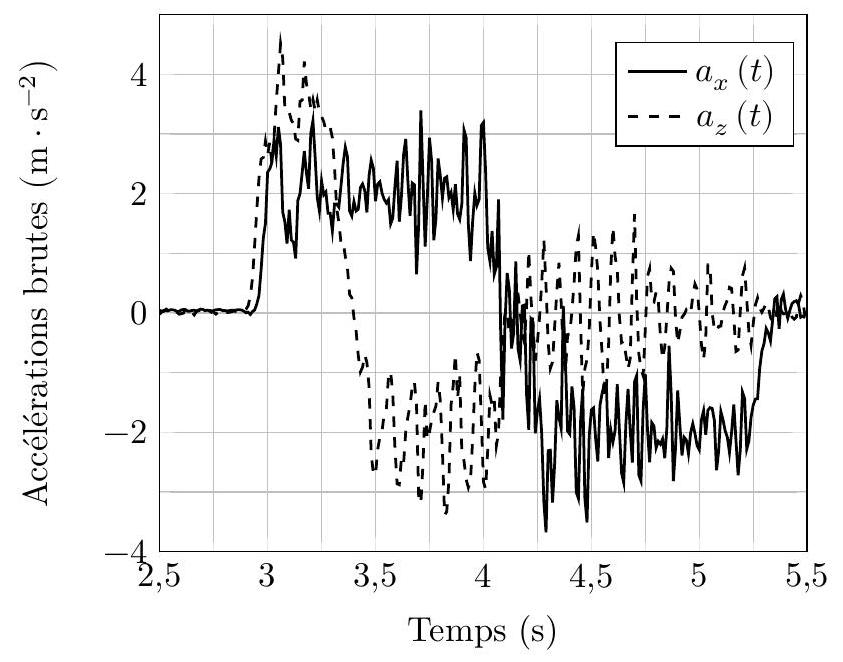
\includegraphics[width=.8\textwidth]{fig_06.jpg}
\caption{\label{fig:06} Déplacement vertical de l'appareil photo pour une perturbation d'amplitude $25 \mathrm{~mm}$ et de fréquences $1 \mathrm{~Hz}$ et $2 \mathrm{~Hz}$ avec une masse $m_{4}=1 \mathrm{~kg}$}
\end{figure}
\fi

%Q 16. 
\question{\label{q:16} Comparer les performances mesurées et simulées (figure~\ref{fig:06}). Peut-on valider le modèle dynamique pour la vérification de l'exigence 1.2. relative à la position de l'appareil photo en mouvement ? Quel phénomène physique pourrait-on prendre en compte pour améliorer le modèle ?}
\ifprof
\begin{corrige}
Pour des perturbations de fréquence de \SI{1}{Hz} ou de \SI{2}{Hz}, la fréquence et les amplitudes des signaux des réponses expérimentales et numériques sont du même ordre de grandeur. (Seule la distorsion du signal est différentes sur les 4 secondes évaluées.)

Au vu des similarités entre les signaux, le modèle dynamique doit donc pouvoir permettre de valider l'exigence~1.2 (Maîtriser la position de l’appareil photo lorsque l’utilisateur marche ou court).

Si vraiment on souhaite améliorer le modèle peut être serait-il possible d'intégrer le frottement éventuel dans les liaisons (qui contribuerait à l'amortissement du système) ou d'intégrer les masses de d'autres pièces.
\end{corrige}
\else
\fi

\subsection{Conclusion}
\ifprof
\else
Pour analyser le respect de l'exigence 1.2. relative à la position en mouvement, des simulations sont réalisées dans plusieurs configurations (figure~\ref{fig:07}).
\fi

%Q 17. 
\question{\label{q:17} Conclure sur la satisfaction de l'exigence 1.2. relative à la position de l'appareil photo en mouvement à l'aide des résultats de simulation (figure~\ref{fig:07}).}
\ifprof
\begin{corrige}
D'après l’exigence 1.2.1.1, le système doit pouvoir << Filtrer les signaux de fréquence comprise entre \SI{1,5}{Hz} et \SI{2,8}{Hz} avec une atténuation supérieure à \SI{16}{dB} et conserver les signaux
de fréquence inférieure à \SI{0,1}{Hz} avec une atténuation inférieure à \SI{3}{dB}. >>

\begin{itemize}
\item Pour une fréquence de \SI{0,1}{Hz}, le déplacement vertical mesuré est de \SI{24}{mm} soit une atténuation de 

$20\log \left( \dfrac{24}{25}\right) = -\SI{0,35}{dB}$. L'atténuation est donc inférieure à \SI{3}{dB}. L'exigence est validée.

\item Pour une fréquence de \SI{1,5}{Hz}, le déplacement vertical mesuré est de \SI{30}{mm} soit une atténuation de 

$20\log \left( \dfrac{30}{25}\right) = \SI{1,58}{dB}$. Le signal est amplifié au lieu d'être atténue. L'exigence n'est pas validée.

\item Pour une fréquence de \SI{2,8}{Hz}, le déplacement vertical mesuré est de \SI{60}{mm}. Le signal est amplifié au lieu d'être atténue. L'exigence n'est pas validée.

\end{itemize}

L'exigence~1.2 n'est donc pas satisfaite. 

\end{corrige}
\else
\fi

\ifprof
\else
Une modification des caractéristiques du ressort pourrait permettre de respecter l'exigence 1.2. relative à la position de l'appareil photo en mouvement. Néanmoins, cette modification impacterait le comportement du système à l'équilibre et ne permettrait plus de respecter l'exigence 1.1. relative à la position d'équilibre. Pour cette raison, une solution technique avec une commande active est présentée et étudiée dans la partie suivante.


\begin{figure}[H]
\centering
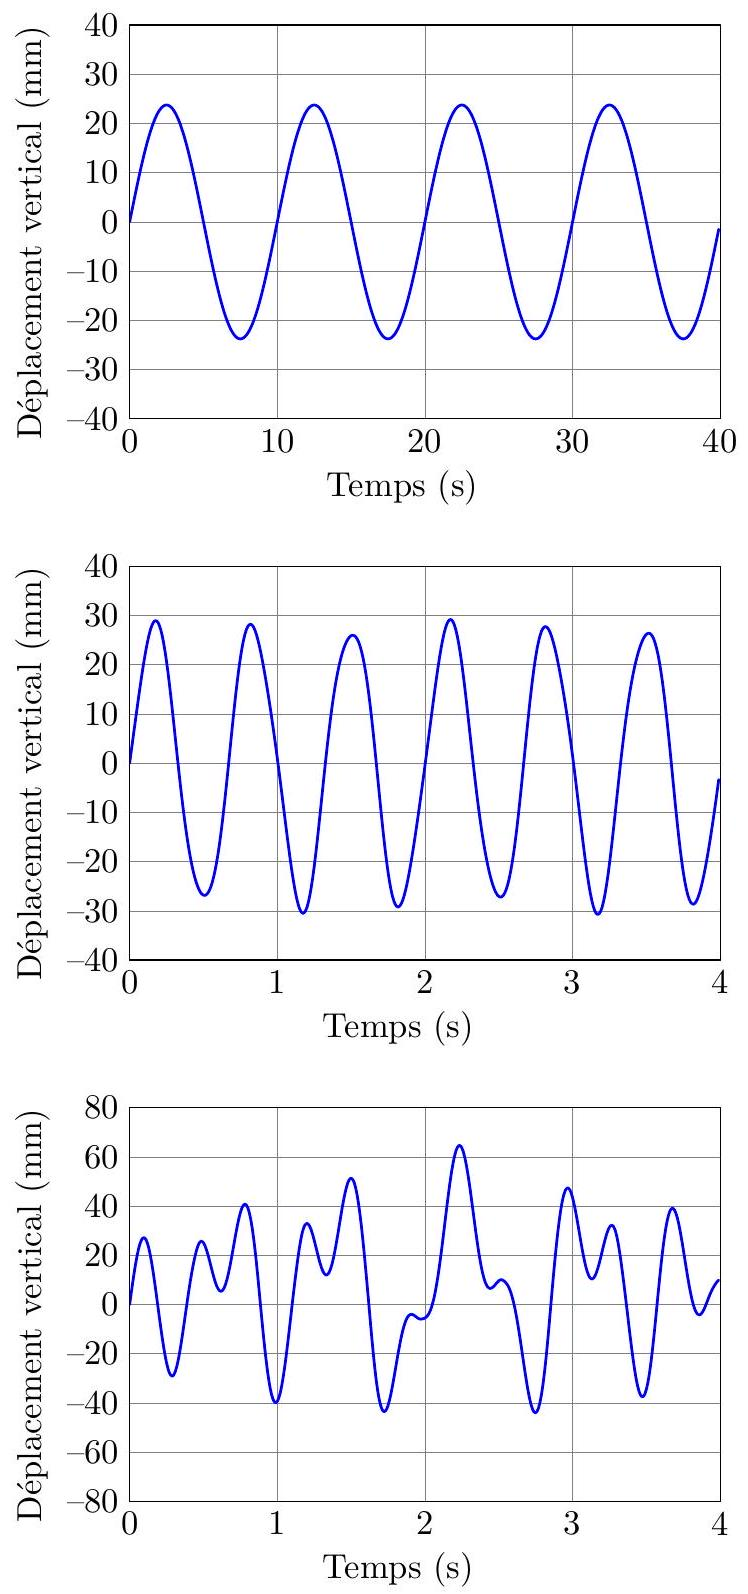
\includegraphics[width=.8\textwidth]{fig_07.jpg}
\caption{\label{fig:07} Simulations du déplacement vertical de l'appareil photo pour une perturbation d'amplitude $25 \mathrm{~mm}$ et de fréquences de $0,1 \mathrm{~Hz}, 1,5 \mathrm{~Hz}$ et $2,8 \mathrm{~Hz}$ avec des masses $m_{4}=0,350 \mathrm{~kg}$ et $m_{4}=1,550 \mathrm{~kg}$
}
\end{figure}
\fi

